%-------------------------------------------------------------------------------
\subsection{Architecture}
%-------------------------------------------------------------------------------
\begin{figure*}[!th]
\begin{center}
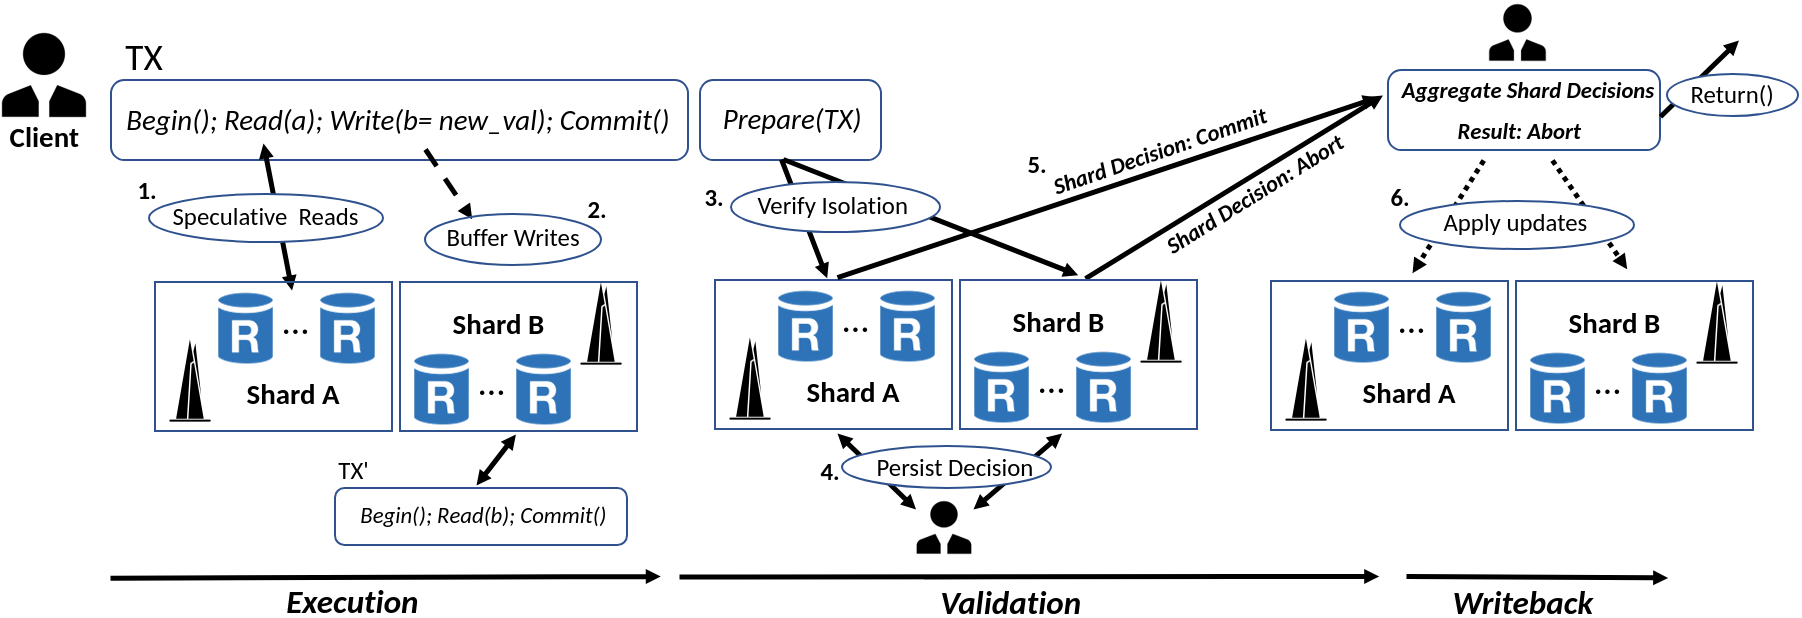
\includegraphics[width= \textwidth]{./figures/Archi.png}
\end{center}
\caption{{\em Transaction Lifecycle}. Clients execute remote reads (1) and buffer writes (2). For Committment, all involved shards verify isolation (3). If there are conflicting transactions (TX'), replicas in a shard (B) vote to Abort. A client persists a decision (4) that serves as Two-Phase-Commit Vote for each shard (5), and Commits a transaction if all shards vote to commit (6).}
\label{fig:Figure1}
\end{figure*}


\sys is designed to be scalable and leaderless. Our architecture reflects this ethos. We briefly summarise it here before going into more detail in the later sections. 
In \sys, clients drive the entire transaction life cycle which can be broken down into three stages as shown in Figure \ref{fig:Figure1}: i) Execution, ii) Validation, and iii) Writeback. 
i) Clients \textit{speculatively execute} transactions themselves, invoking only remote read procedure calls and buffering writes locally. Transactions may read and write arbitrarily and can span several data partitions (shards). Moreover, different clients may execute transactions concurrently, performing reads in different order at (a subset of) replicas within each shard. 
ii) Since execution is speculative, and clients are unaware of potential concurrency, they must \textit{validate} their transaction execution for Isolation correctness in order to be able to commit. Intuitively, if there are no conflicting concurrent transactions, and a clients transaction observed a consistent snapshot of the database state then it may commit, and otherwise must retry or abort its transaction. Validation too, is client driven, and may happen in different order, both across different shards, as well as across replicas within each shard. For every relevant shard, a client must query potentially inconsistent replicas for their commitment vote, reconcile divergent votes into a single per-shard decision that maintains Isolation, and make this decision durable to avoid replay of contradictory decisions. 
iii) Lastly, a client aggregates all shard decisions in atomic commit fashion and returns to the application. Asynchronously, it \textit{writes back} the decision to all involved replicas who apply the transaction to their local database state.

Next, we outline the protocols for Execution, Validation and Writeback respectively. 



